\documentclass[11pt]{article}
\usepackage[margin=2.2cm]{geometry}
\usepackage{fontspec}
\setmainfont{STIX Two Text}
\usepackage{unicode-math}
\setmathfont{STIX Two Math}
\usepackage{graphicx,booktabs,enumitem,hyperref,float}
\setlist{nosep,leftmargin=1.4em}
\setlength{\parskip}{4pt}
\title{Two-color excitation with focused optical pulses:\\ background, replication, and how it connects to the current work}
\date{23 September 2026}
\author{}
\begin{document}
\maketitle
\vspace{-2.5em}

\noindent The new direction: two beams of different color, each tightly focused, excite a sample only where
they overlap in space and time. This document builds the physics from Maxwell's equations up to that
signal (Part I), reports the replication of the three low-NA papers the work starts from (Part II), and
connects both to the Richards--Wolf pulsed-focus work already done (Part III). Every citation was checked
against its DOI record (Crossref) or ISBN.

\part*{I. Background from first principles}

\section{From Maxwell's equations to the Helmholtz equation}
In a source-free, linear, isotropic medium of refractive index $n$, Maxwell's equations give
$\nabla\cdot\mathbf E=0$ and $\nabla^2\mathbf E-(n^2/c^2)\,\partial_t^2\mathbf E=0$
\cite{BornWolf, NovotnyHecht}. For monochromatic light,
$\mathbf E(\mathbf r,t)=\mathrm{Re}[\mathbf E(\mathbf r)e^{-i\omega t}]$, and the time dependence drops out:
\[
\nabla^2\mathbf E+k^2\mathbf E=0,\qquad \nabla\cdot\mathbf E=0,\qquad k=\frac{n\omega}{c}=\frac{2\pi n}{\lambda}.
\]
The first is the Helmholtz equation; the second, transversality, is what makes the field a vector problem.
Detectors and molecules respond to the cycle-averaged intensity, $I\propto|\mathbf E|^2$.

\section{Plane waves and the angular spectrum}
The simplest solution is a plane wave, $\mathbf E=\mathbf E_0\,e^{i\mathbf k\cdot\mathbf r}$ with
$|\mathbf k|=k$. Transversality forces $\mathbf k\cdot\mathbf E_0=0$: \emph{the field of every plane wave is
perpendicular to its own direction}. Any source-free field in a half-space can be written as a superposition of
such plane waves, its angular spectrum \cite{Goodman, NovotnyHecht}. A focus is exactly this: many plane waves,
arriving from many directions, adding up at one point. Because each wave must stay transverse to its own
direction, waves arriving at large angles necessarily carry a component along the optical axis.

\section{A lens and its focus: the Debye integral}
A lens turns an incoming plane wave into a spherical wave converging on the focus. Huygens' principle, made
quantitative by Kirchhoff, propagates that wave to the focal region \cite{BornWolf, Goodman}. Debye
\cite{Debye} showed that when the aperture is many wavelengths across and the Fresnel number
$a^2/\lambda f$ is large (the condition Lim \& Saloma state, \cite{LS02} p.~122), the focal field is a
superposition of plane waves whose directions fill the cone the aperture subtends at the focus, each weighted
by the field on the aperture. Wolf put this in integral form \cite{Wolf59}. For a scalar field and a pupil
that depends only on the angle $\vartheta$ from the axis,
\[
\begin{aligned}
U(r,z)&=\int_0^{\alpha}\!\!\int_0^{2\pi} a(\vartheta)\,e^{ik(r\sin\vartheta\cos(\varphi-\psi)+z\cos\vartheta)}
\sin\vartheta\,d\varphi\,d\vartheta\\
&=2\pi\!\int_0^{\alpha} a(\vartheta)\,J_0(kr\sin\vartheta)\,e^{ikz\cos\vartheta}\sin\vartheta\,d\vartheta,
\end{aligned}
\]
where $\sin\alpha=\mathrm{NA}/n$, $\sin\vartheta\,d\vartheta\,d\varphi$ is the solid-angle element, and the
azimuthal integral is the Bessel identity
\[\int_0^{2\pi}e^{iv\cos(\varphi-\psi)}\,d\varphi=2\pi J_0(v).\]

\section{\texorpdfstring{The aplanatic lens: where $\sqrt{\cos\vartheta}$ comes from}{The aplanatic lens: where the square root of cos theta comes from}}
A well-corrected (aplanatic) lens obeys the sine condition: a ray entering at height $h$ leaves toward the
focus at the angle $\vartheta$ with $h=f\sin\vartheta$ (Fig.~\ref{fig:geom}) \cite{BornWolf, RichardsWolf}.
Energy conservation then fixes the amplitude on the reference sphere. The power through a pupil ring,
$|E_{\text{in}}|^2\,2\pi h\,dh$, must equal the power through the matching band of the sphere,
$|E_{\text{sph}}|^2\,2\pi f^2\sin\vartheta\,d\vartheta$. With $dh=f\cos\vartheta\,d\vartheta$,
\[
|E_{\text{sph}}|^2=|E_{\text{in}}|^2\cos\vartheta
\quad\Longrightarrow\quad a(\vartheta)=A(\vartheta)\sqrt{\cos\vartheta},
\]
where $A(\vartheta)$ is the input beam profile: 1 for uniform illumination,
$\exp(-\alpha_t\sin^2\vartheta/\sin^2\alpha)$ for the truncated Gaussian of the current work.

\begin{figure}[H]\centering
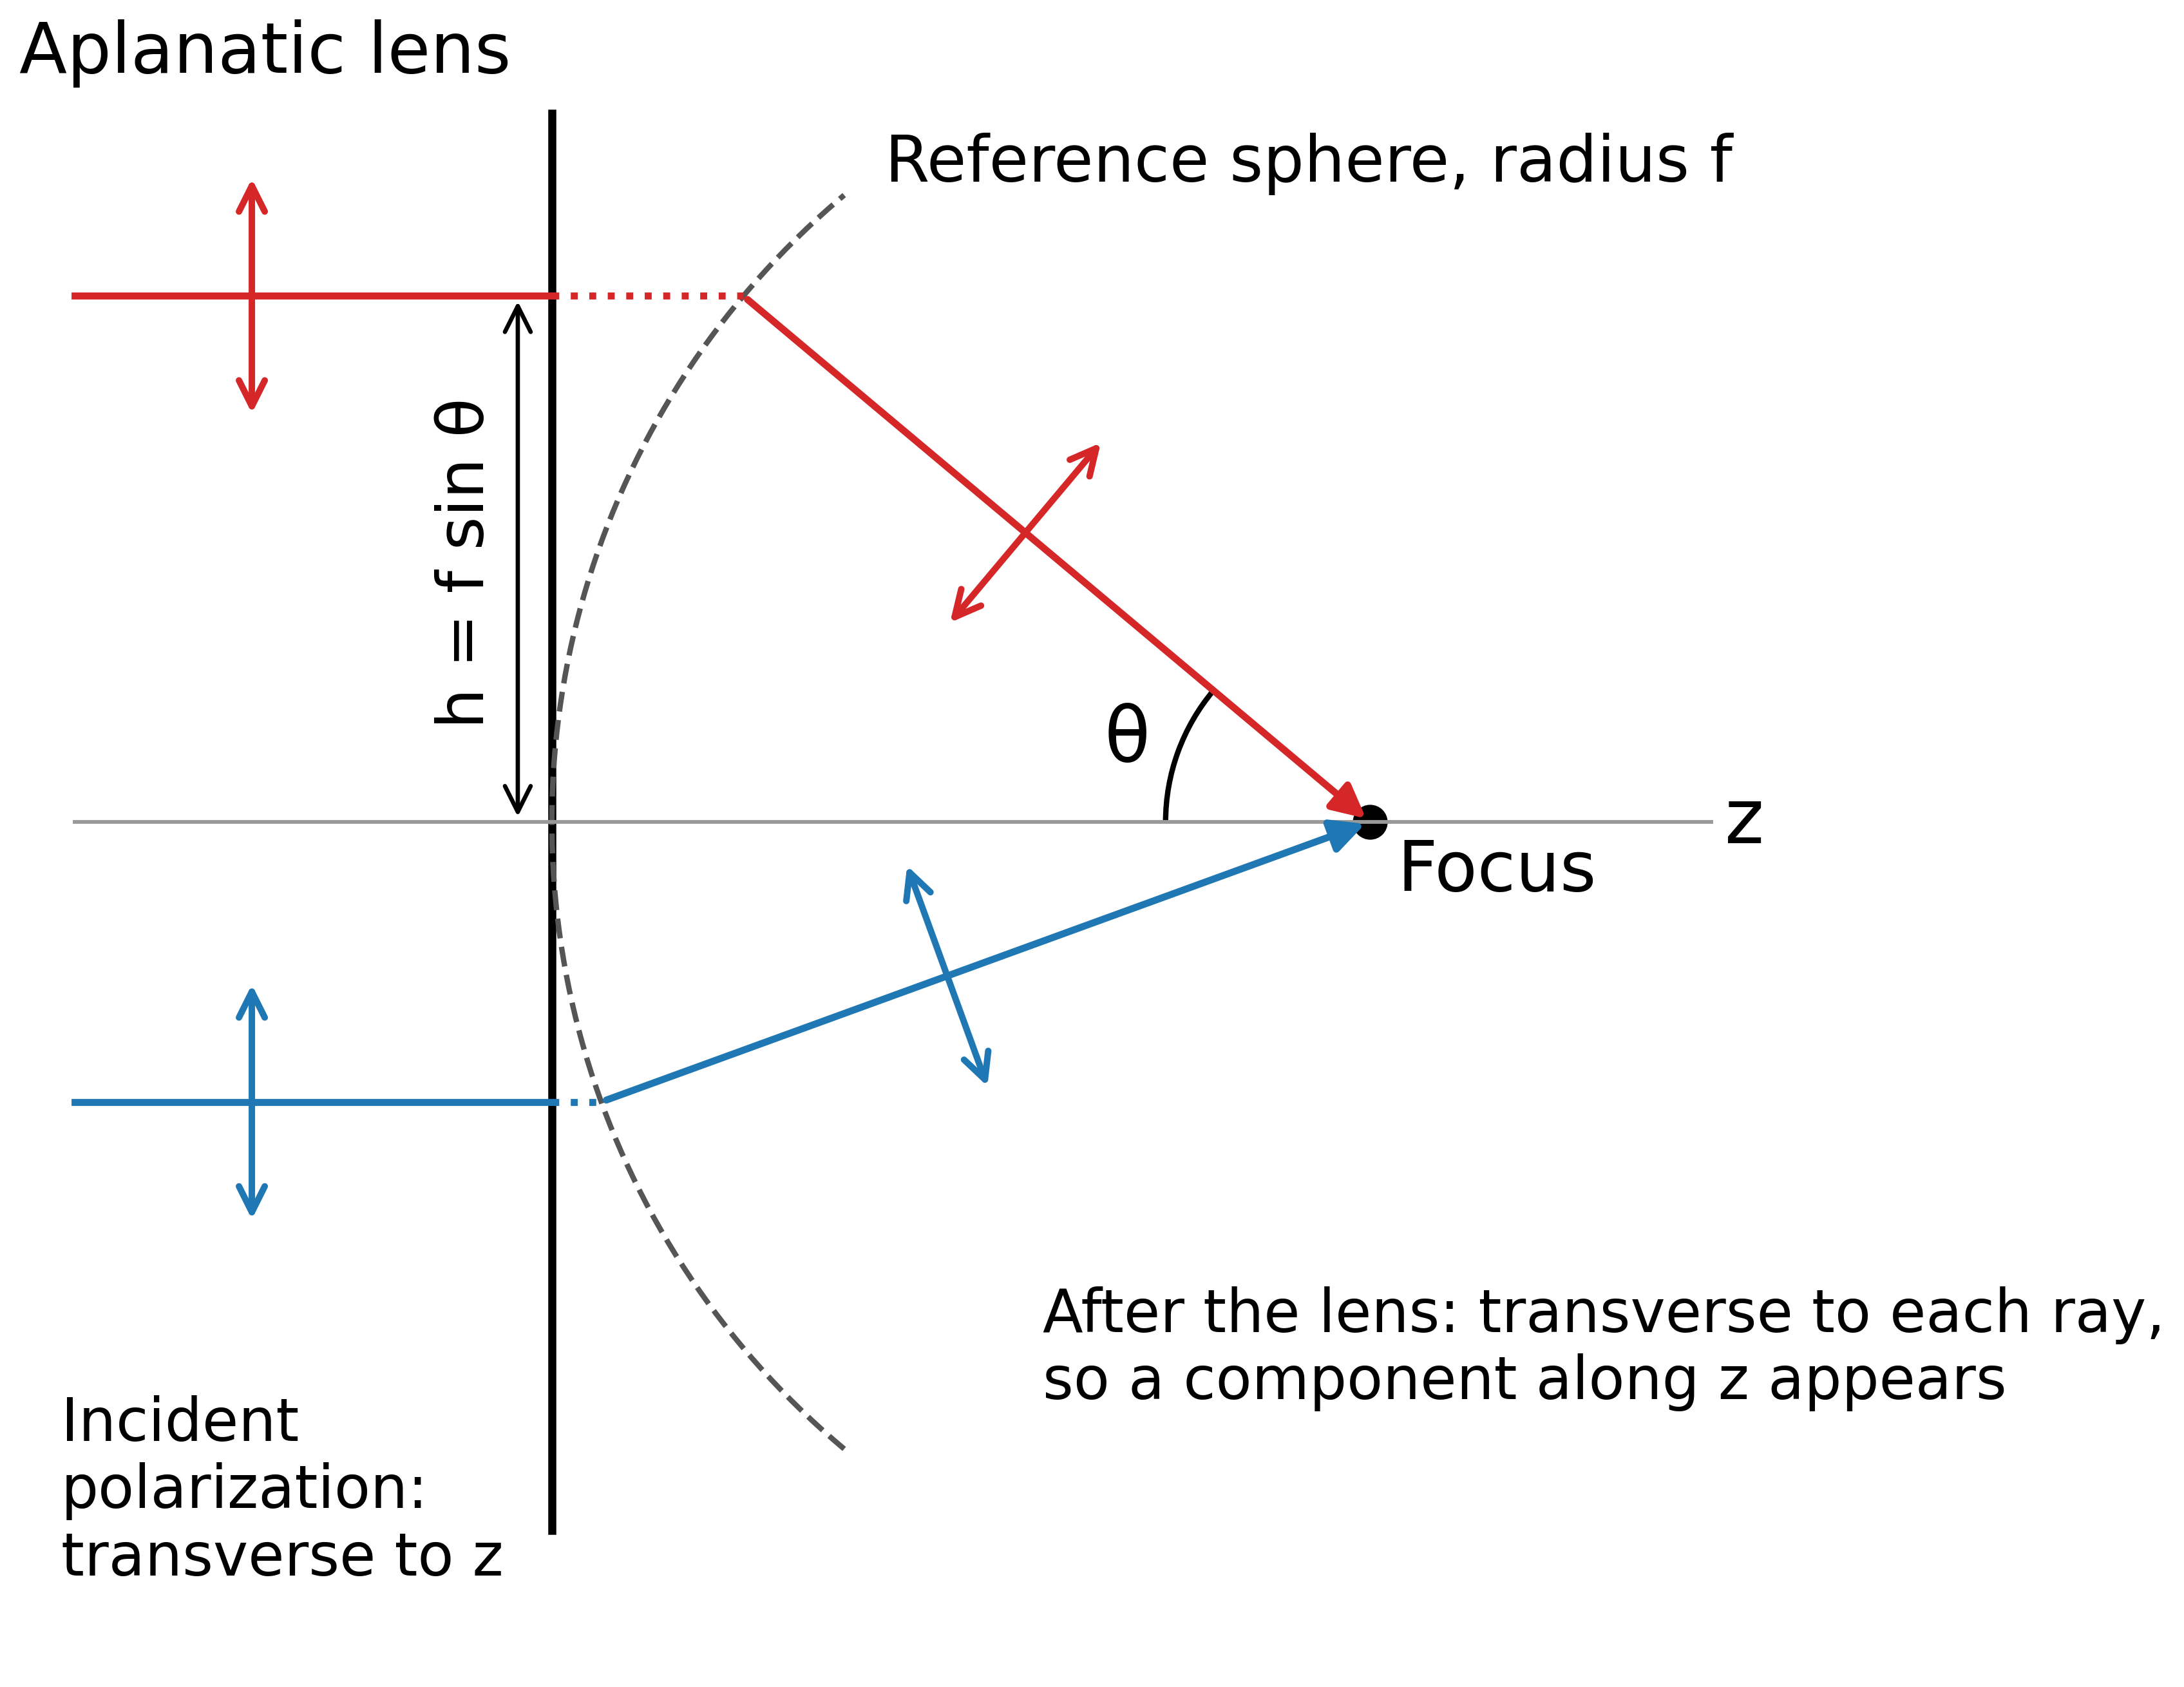
\includegraphics[width=0.66\linewidth]{bg_focusing_geometry.png}
\caption{Aplanatic focusing. Each ray leaves the lens at height $h=f\sin\vartheta$ and travels along a radius of
the reference sphere. Its polarization, transverse to $z$ before the lens, must be transverse to the ray
afterwards, so rays at large $\vartheta$ carry a field component along $z$.}\label{fig:geom}
\end{figure}

\section{Polarization through the lens: Richards--Wolf}
Richards and Wolf \cite{RichardsWolf} carried the vector field through the aplanatic lens. For $x$-polarized
input, the ray at $(\vartheta,\varphi)$ reaches the reference sphere with unit field \cite{NovotnyHecht}
\[
\hat{\mathbf e}(\vartheta,\varphi)=\big(\cos\vartheta\cos^2\varphi+\sin^2\varphi,\;
(\cos\vartheta-1)\sin\varphi\cos\varphi,\; -\sin\vartheta\cos\varphi\big).
\]
The component along the ray's radial (meridional) direction is tilted with the ray; the azimuthal component is
unchanged. Rewriting the $x$ component as
$\tfrac12(1+\cos\vartheta)-\tfrac12(1-\cos\vartheta)\cos2\varphi$ and integrating each term over $\varphi$ with
$\int_0^{2\pi}\cos(m\varphi)\,e^{iv\cos(\varphi-\psi)}d\varphi=2\pi i^m J_m(v)\cos(m\psi)$ gives the focal field
\cite{RichardsWolf, Rom03}:
\[
E_x=-i(I_0+I_2\cos2\psi),\qquad E_y=-iI_2\sin2\psi,\qquad E_z=-2iI_1\cos\psi,
\]
\[
I_m=\int_0^{\alpha}A(\vartheta)\sqrt{\cos\vartheta}\,\sin\vartheta\;g_m(\vartheta)\,J_m(kr\sin\vartheta)\,
e^{ikz\cos\vartheta}\,d\vartheta,\qquad g_0=1+\cos\vartheta,\; g_1=\sin\vartheta,\; g_2=1-\cos\vartheta .
\]
$I_0$ is the familiar focusing term; $I_2$ breaks the circular symmetry of the spot; $I_1$ is the longitudinal
field $E_z$. This is the field the current work computes (Romallosa replication, 472.8\,nm checkpoint).

\section{The low-NA limit: the model the two-color papers use}
For a small cone, $\vartheta\ll1$: $\sin\vartheta\approx\vartheta$, $\cos\vartheta\approx1-\vartheta^2/2$, so
$g_0\to2$, $g_1,g_2\to0$ ($E_y$ and $E_z$ vanish), $\sqrt{\cos\vartheta}\to1$, and the phase becomes
quadratic. With $\rho=\vartheta/\alpha$,
\[
U(u,v)\propto e^{ikz}\;2\!\int_0^1 J_0(v\rho)\,e^{-iu\rho^2/2}\rho\,d\rho,\qquad
u=k\Big(\frac{\mathrm{NA}}{n}\Big)^2 z,\quad v=\frac{2\pi}{\lambda}\,\mathrm{NA}\,r,
\]
the scalar field expressed by Lommel functions \cite{BornWolf}. Its focal-plane profile is the Airy pattern
and its axial profile $\mathrm{sinc}^2(u/4)$. All three two-color papers use it \cite{CS00, LS02, LS03}.
Figure~\ref{fig:na} shows what it misses.

\begin{figure}[H]\centering
\includegraphics[width=\linewidth]{bg_low_high_na.png}
\caption{Richards--Wolf against the paraxial scalar field, 750\,nm, $n=1.3$, uniform input, $x$-polarized.
At NA 0.5 the two nearly coincide transversely; $E_z$ is 2\% of the peak. At NA 1.2 the spot is elongated along
the polarization, $E_z$ reaches 16\% of the peak off axis, and the scalar model is visibly wrong. Axially the
Richards--Wolf focus is 4\% shorter than the paraxial one at NA 0.5 and much shorter at NA 1.2, because the
exact phase $kz\cos\vartheta$ departs from its quadratic approximation.}\label{fig:na}
\end{figure}

\noindent The current work puts the 1\% focal-width departure between scalar and vector theory at NA
$\approx0.45$, so the papers' NA 0.5 sits at the edge of their model's validity.

\section{Light and matter: one, two, and two-color excitation}
\textbf{One photon.} A molecule absorbs a photon of energy $\hbar\omega$ at a rate proportional to $|E|^2=I$.
Integrated over any plane through the beam, $\int I\,dA$ is the beam power, the same in every plane: one-photon
fluorescence comes from the whole cone, not only the focus (Fig.~\ref{fig:nl}).

\textbf{Two photons.} Göppert-Mayer showed that two photons can be absorbed together through a short-lived
virtual state, at a rate proportional to $I^2$ \cite{GoeppertMayer}. Now $\int I^2\,dA$ falls away from the
focus, so excitation is confined to the focal volume. This is the basis of two-photon microscopy
\cite{Denk90}.

\textbf{Two colors.} The two photons can come from different beams, $\hbar\omega_1+\hbar\omega_2=\hbar\omega_e$,
i.e.\ $1/\lambda_e=1/\lambda_1+1/\lambda_2$ (Fig.~\ref{fig:levels}); two-color two-photon excitation has been
observed experimentally \cite{Lakowicz96}. The rate is proportional to the product of the two intensities
\cite{CS00}:
\[
F_{2c}(P)=\kappa\,I_1(P)\,I_2(P).
\]
It is zero wherever either beam is absent, so fluorescence exists only where the two foci overlap.
Each beam alone can still drive ordinary two-photon absorption if its own photons suffice, which is why
probes are chosen to suppress it \cite{LS03}.

\begin{figure}[H]\centering
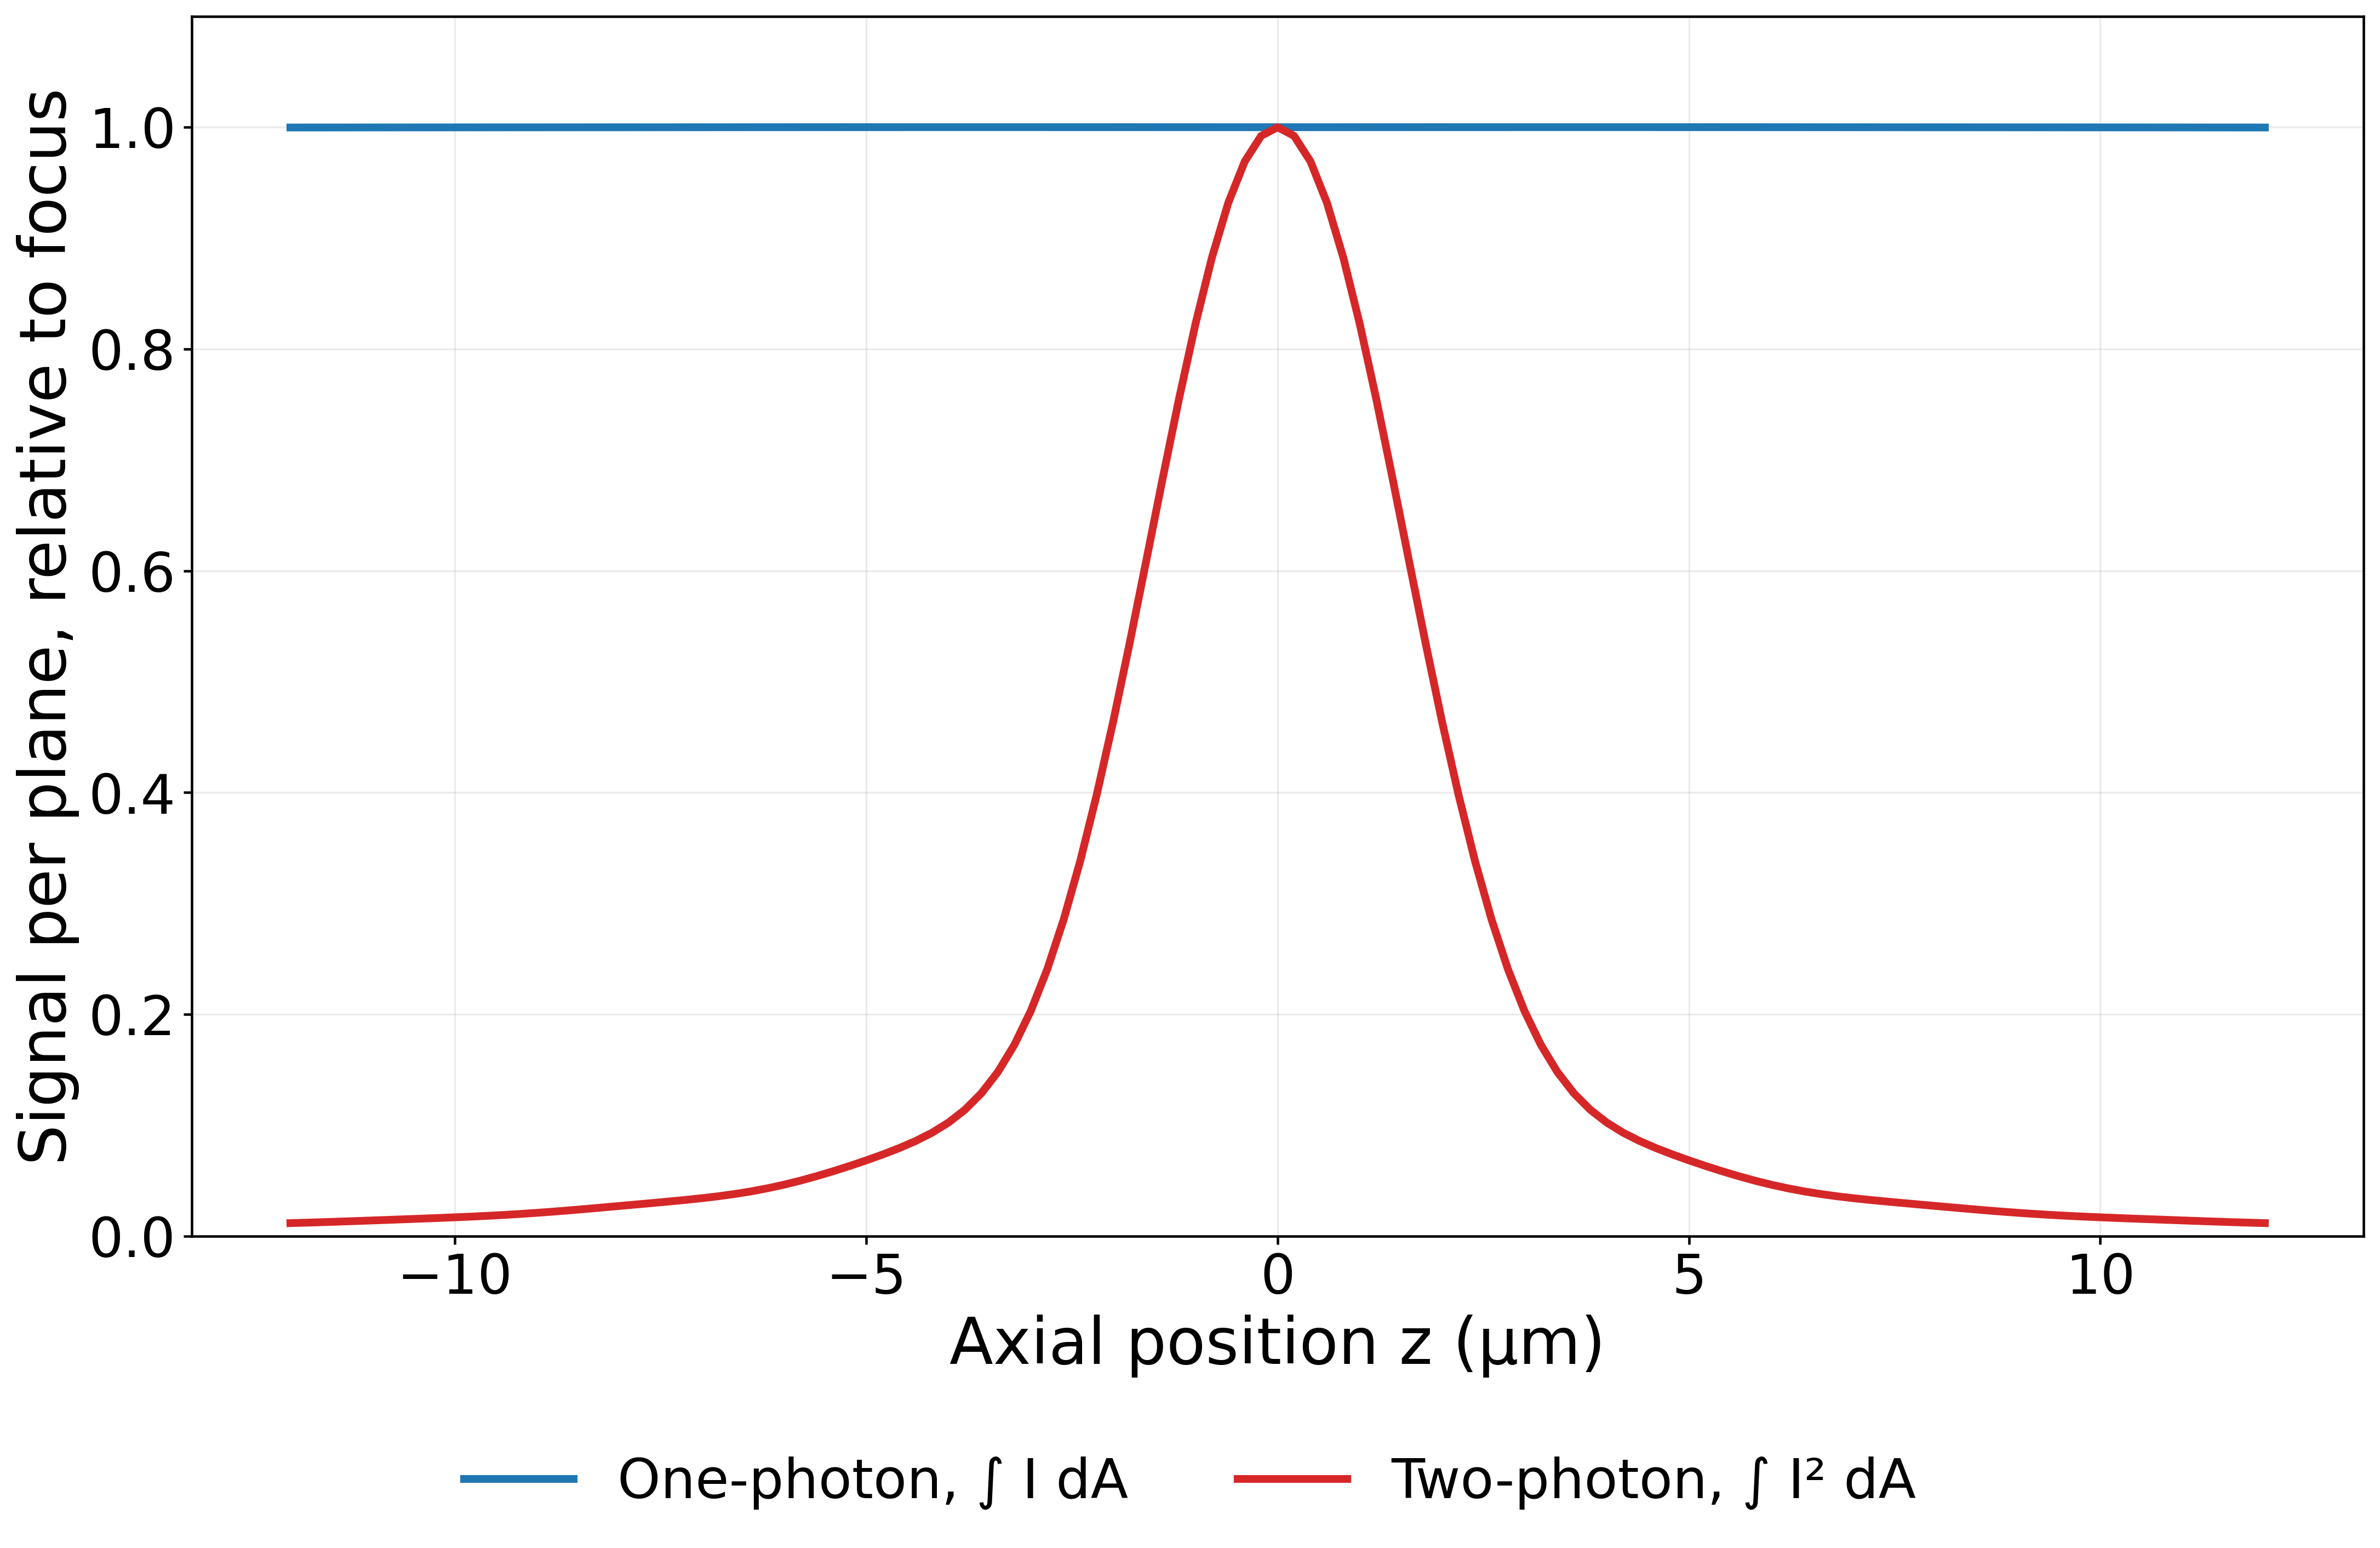
\includegraphics[width=0.46\linewidth]{bg_nonlinear.png}\hfill
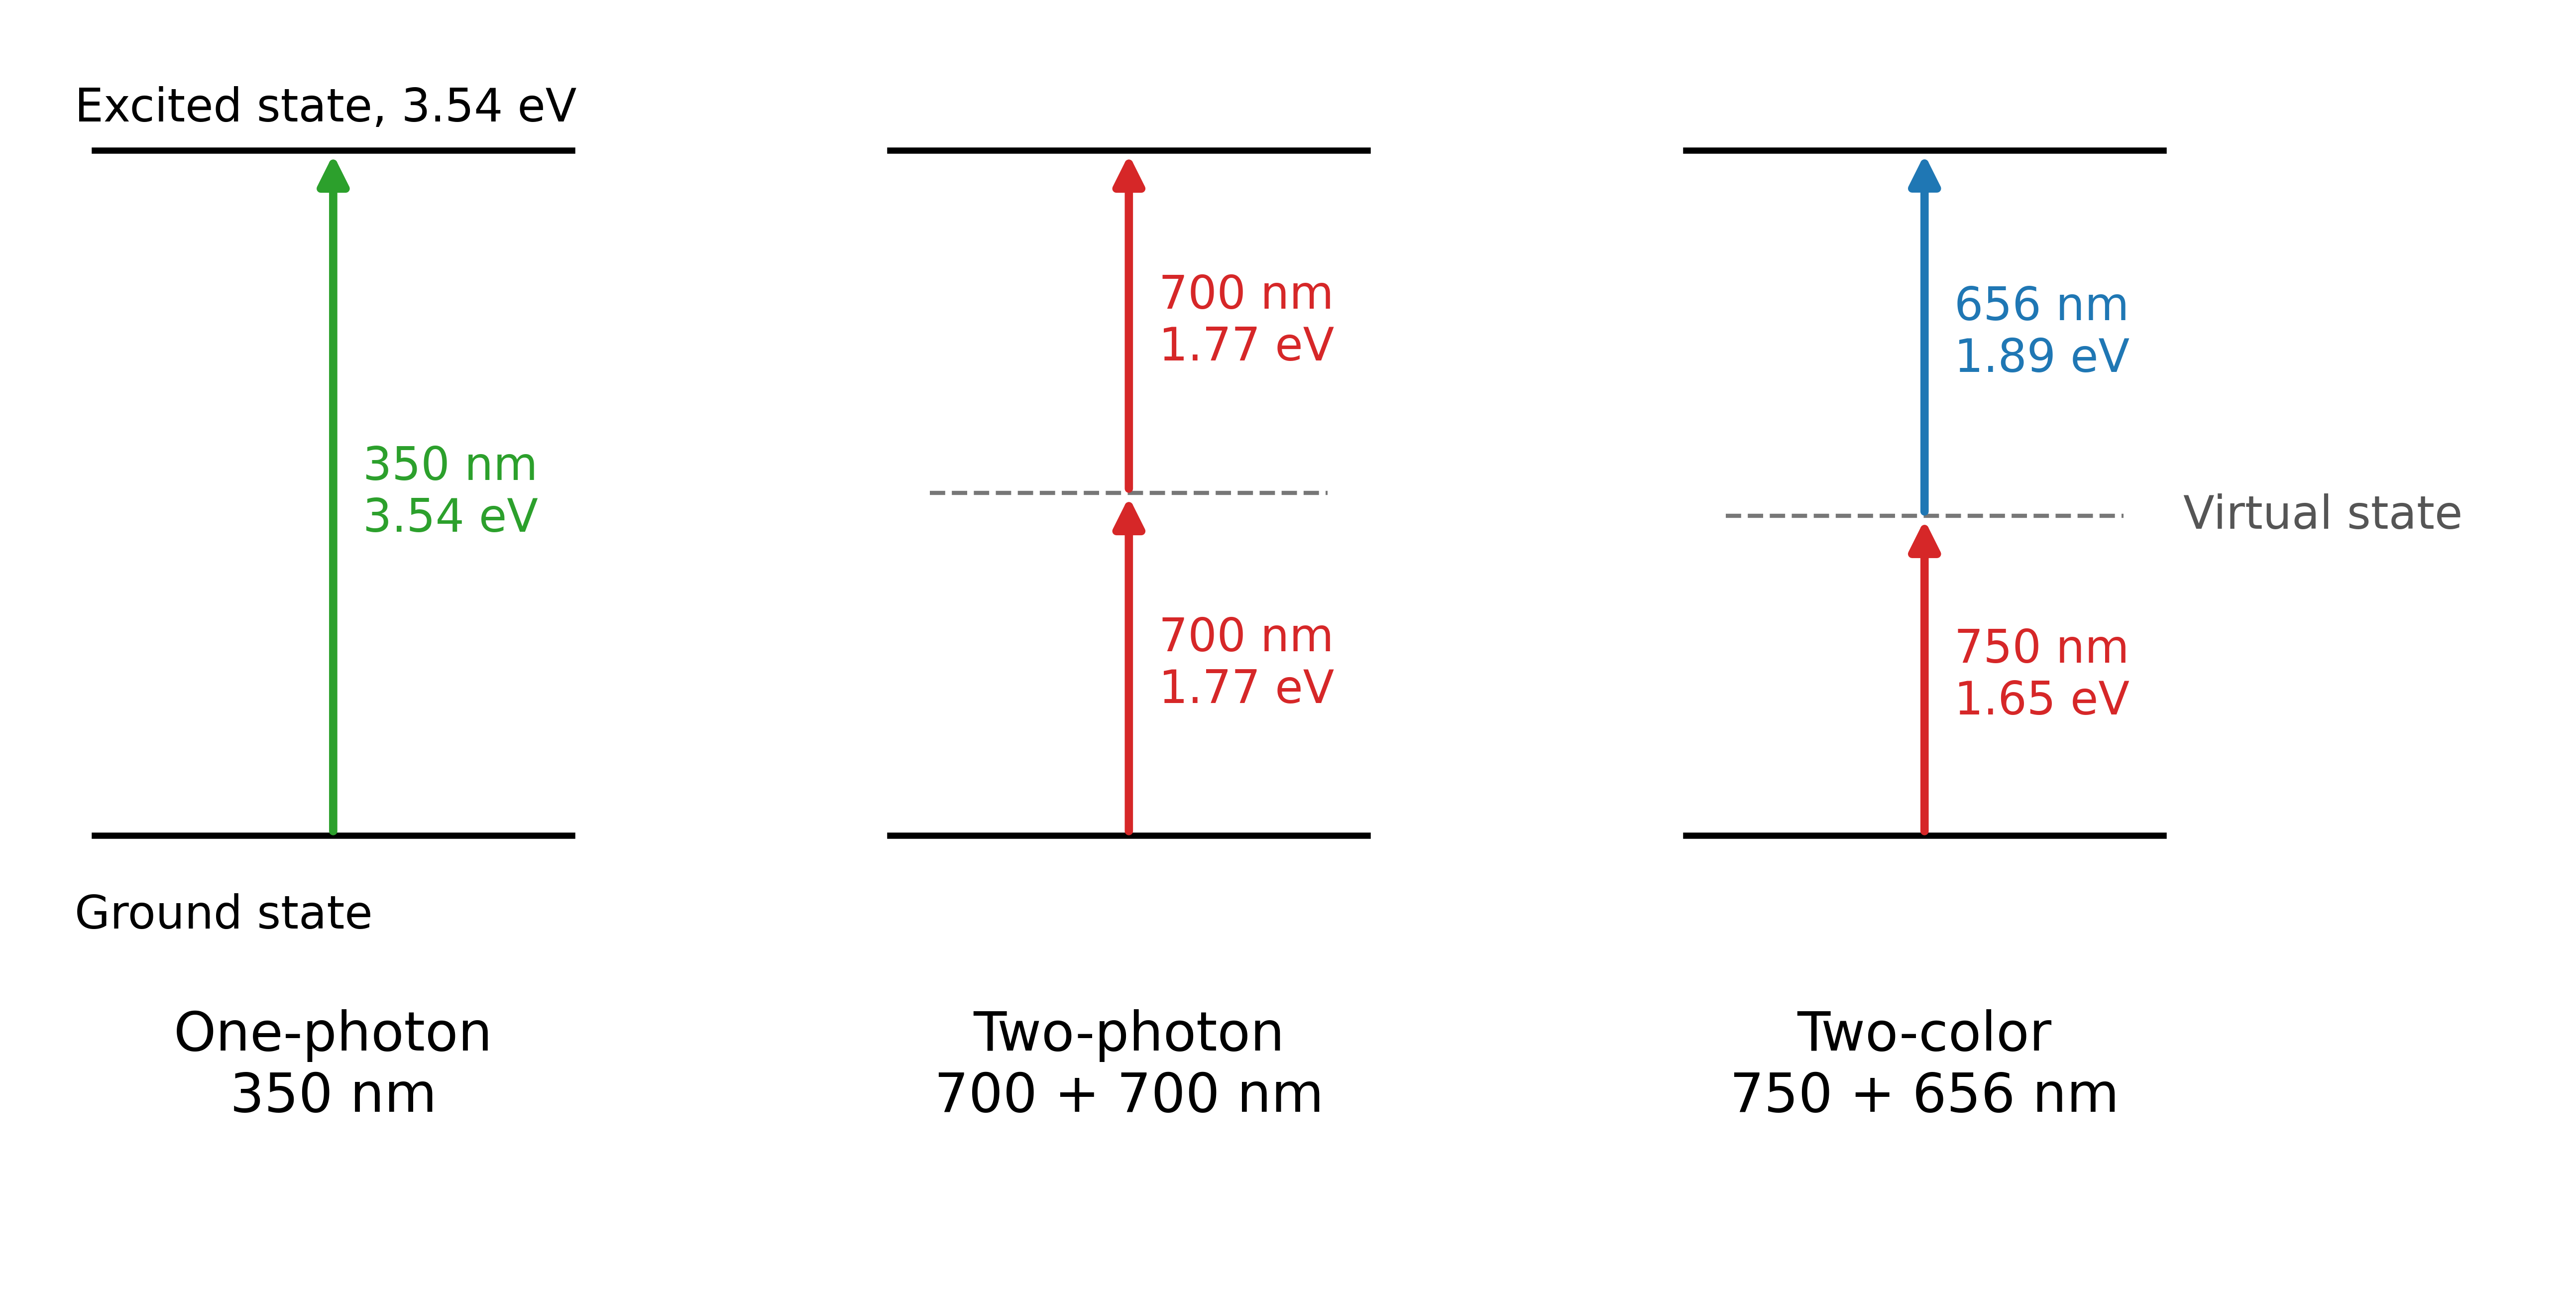
\includegraphics[width=0.52\linewidth]{bg_energy_levels.png}
\caption{Left: signal per plane against distance from focus (paraxial, NA 0.5, 700\,nm). One-photon excitation
is the same in every plane; two-photon excitation is confined to the focus. Right: the three transitions to
the same 3.54\,eV state.}\label{fig:nl}\label{fig:levels}
\end{figure}

\section{Why two colors do not interfere and two photons of one color do}
With both beams present, the total field is
$\mathbf E_1e^{-i\omega_1t}+\mathbf E_2e^{-i\omega_2t}$, and
\[
|\mathbf E|^2=|\mathbf E_1|^2+|\mathbf E_2|^2+2\,\mathrm{Re}\big[\mathbf E_1\cdot\mathbf E_2^*\,e^{-i(\omega_1-\omega_2)t}\big].
\]
For one color ($\omega_1=\omega_2$) the cross term is steady and depends on the relative phase: the two beams
interfere, and the two-photon rate is $F_{2p}=\kappa'|U_1+U_2|^4$ \cite{CS00}, which is why two-beam 2PE shows
fringes. For two colors the cross term oscillates at the difference frequency (57\,THz, a 17.5\,fs period for
750 and 656\,nm) and averages away (Fig.~\ref{fig:beat}). This holds only if the two spectra do not overlap
\cite{CS00}. In the vector case the cross term is $\mathbf E_1\cdot\mathbf E_2^*$: beams polarized at right
angles do not interfere at all, so polarization becomes a design variable the scalar papers cannot see.

\begin{figure}[H]\centering
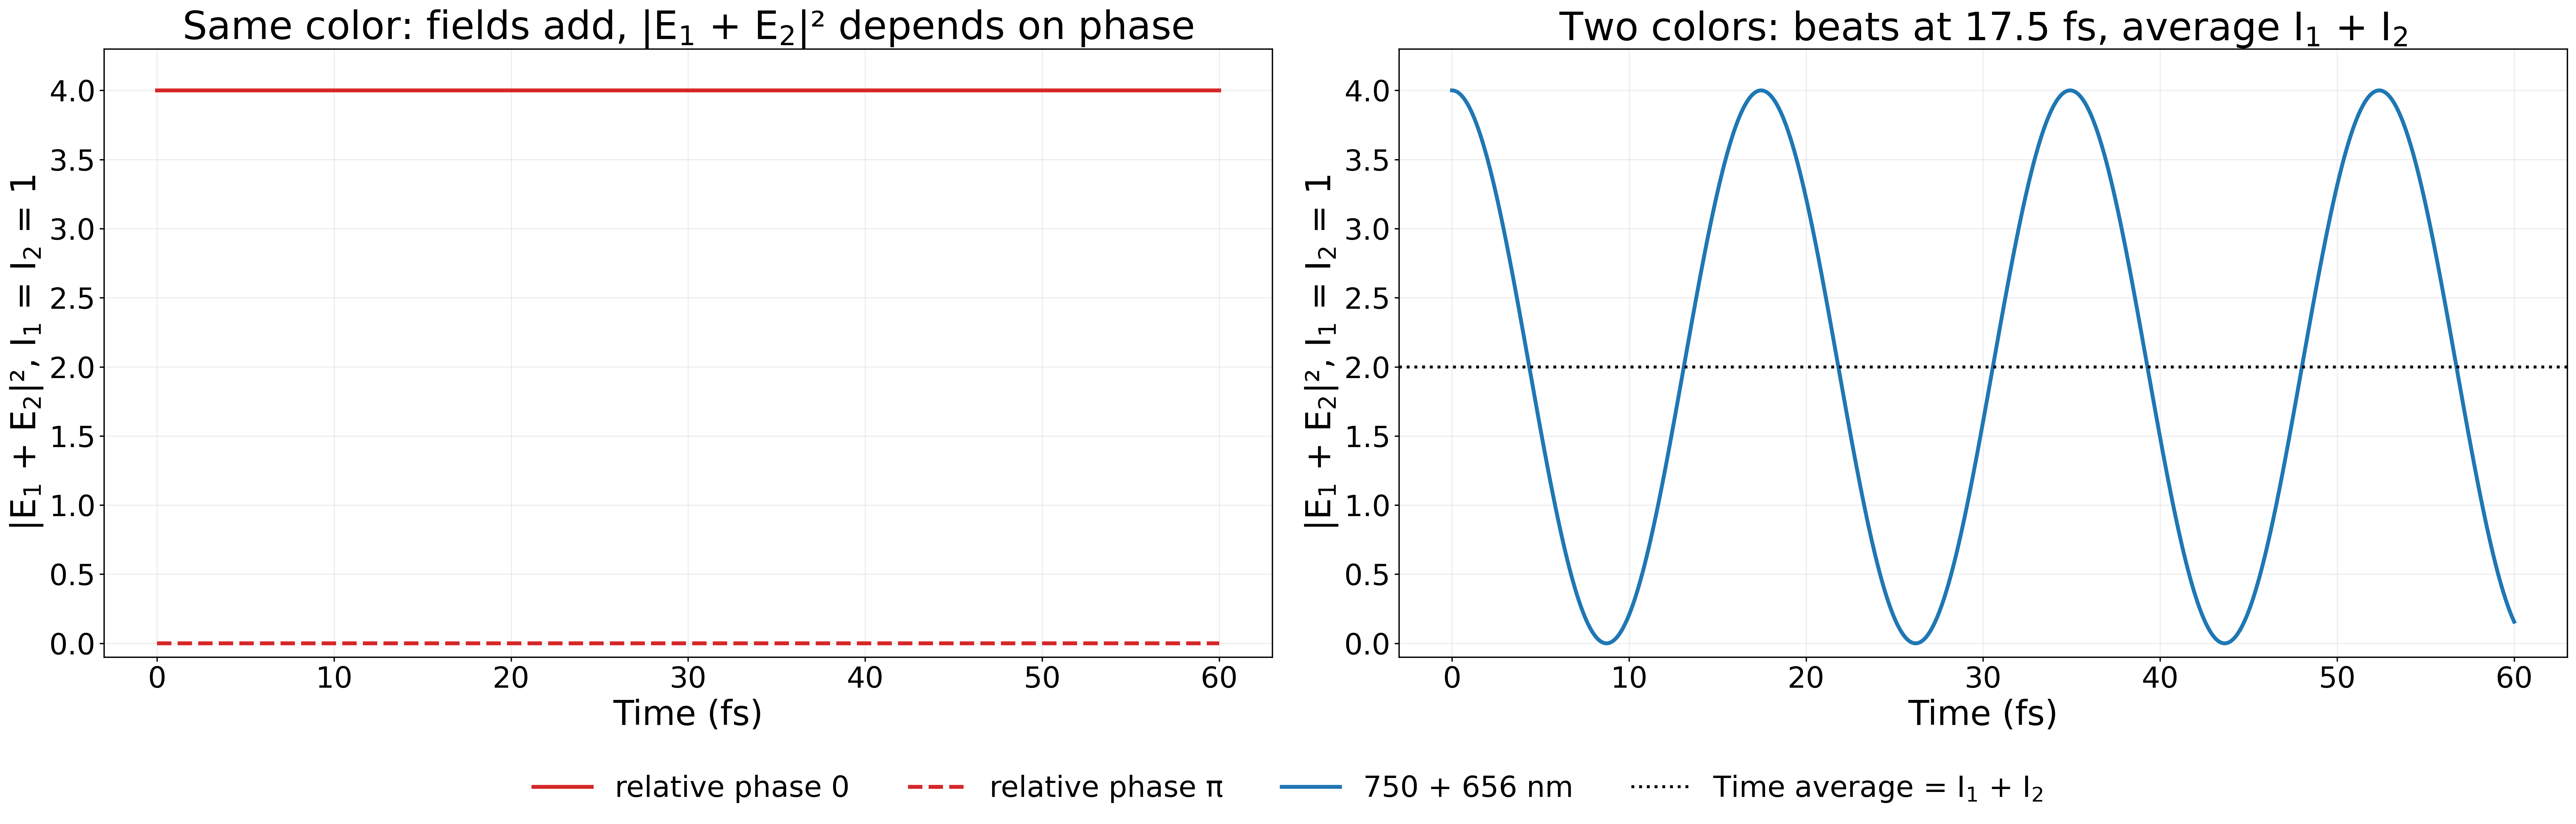
\includegraphics[width=\linewidth]{bg_beating.png}
\caption{$|\mathbf E_1+\mathbf E_2|^2$ over time for equal intensities. Same color: steady, and set by the
relative phase (0 to 4). Two colors: beats at the difference frequency, averaging to $I_1+I_2$.}\label{fig:beat}
\end{figure}

\section{Two beams at an angle}
Placing the second lens at an angle $\theta$ to the first is the idea of theta microscopy \cite{Lindek99};
$\theta=\pi$, two opposed lenses, is the 4Pi arrangement \cite{Hell92}. Beam 2 is computed in its own frame and
rotated into the lab frame (Fig.~\ref{fig:setup}); in the vector case its field vector, including its own
$E_z$, rotates with it. Two cones of half-angle $\alpha$ meeting at $\theta=\pi/2$ fit only if
$\alpha\le45^\circ$: NA $\le n/\sqrt2$, which is 0.71 at $n=1$ (\cite{CS00} p.~34) and 0.92 at $n=1.3$.

\begin{figure}[H]\centering
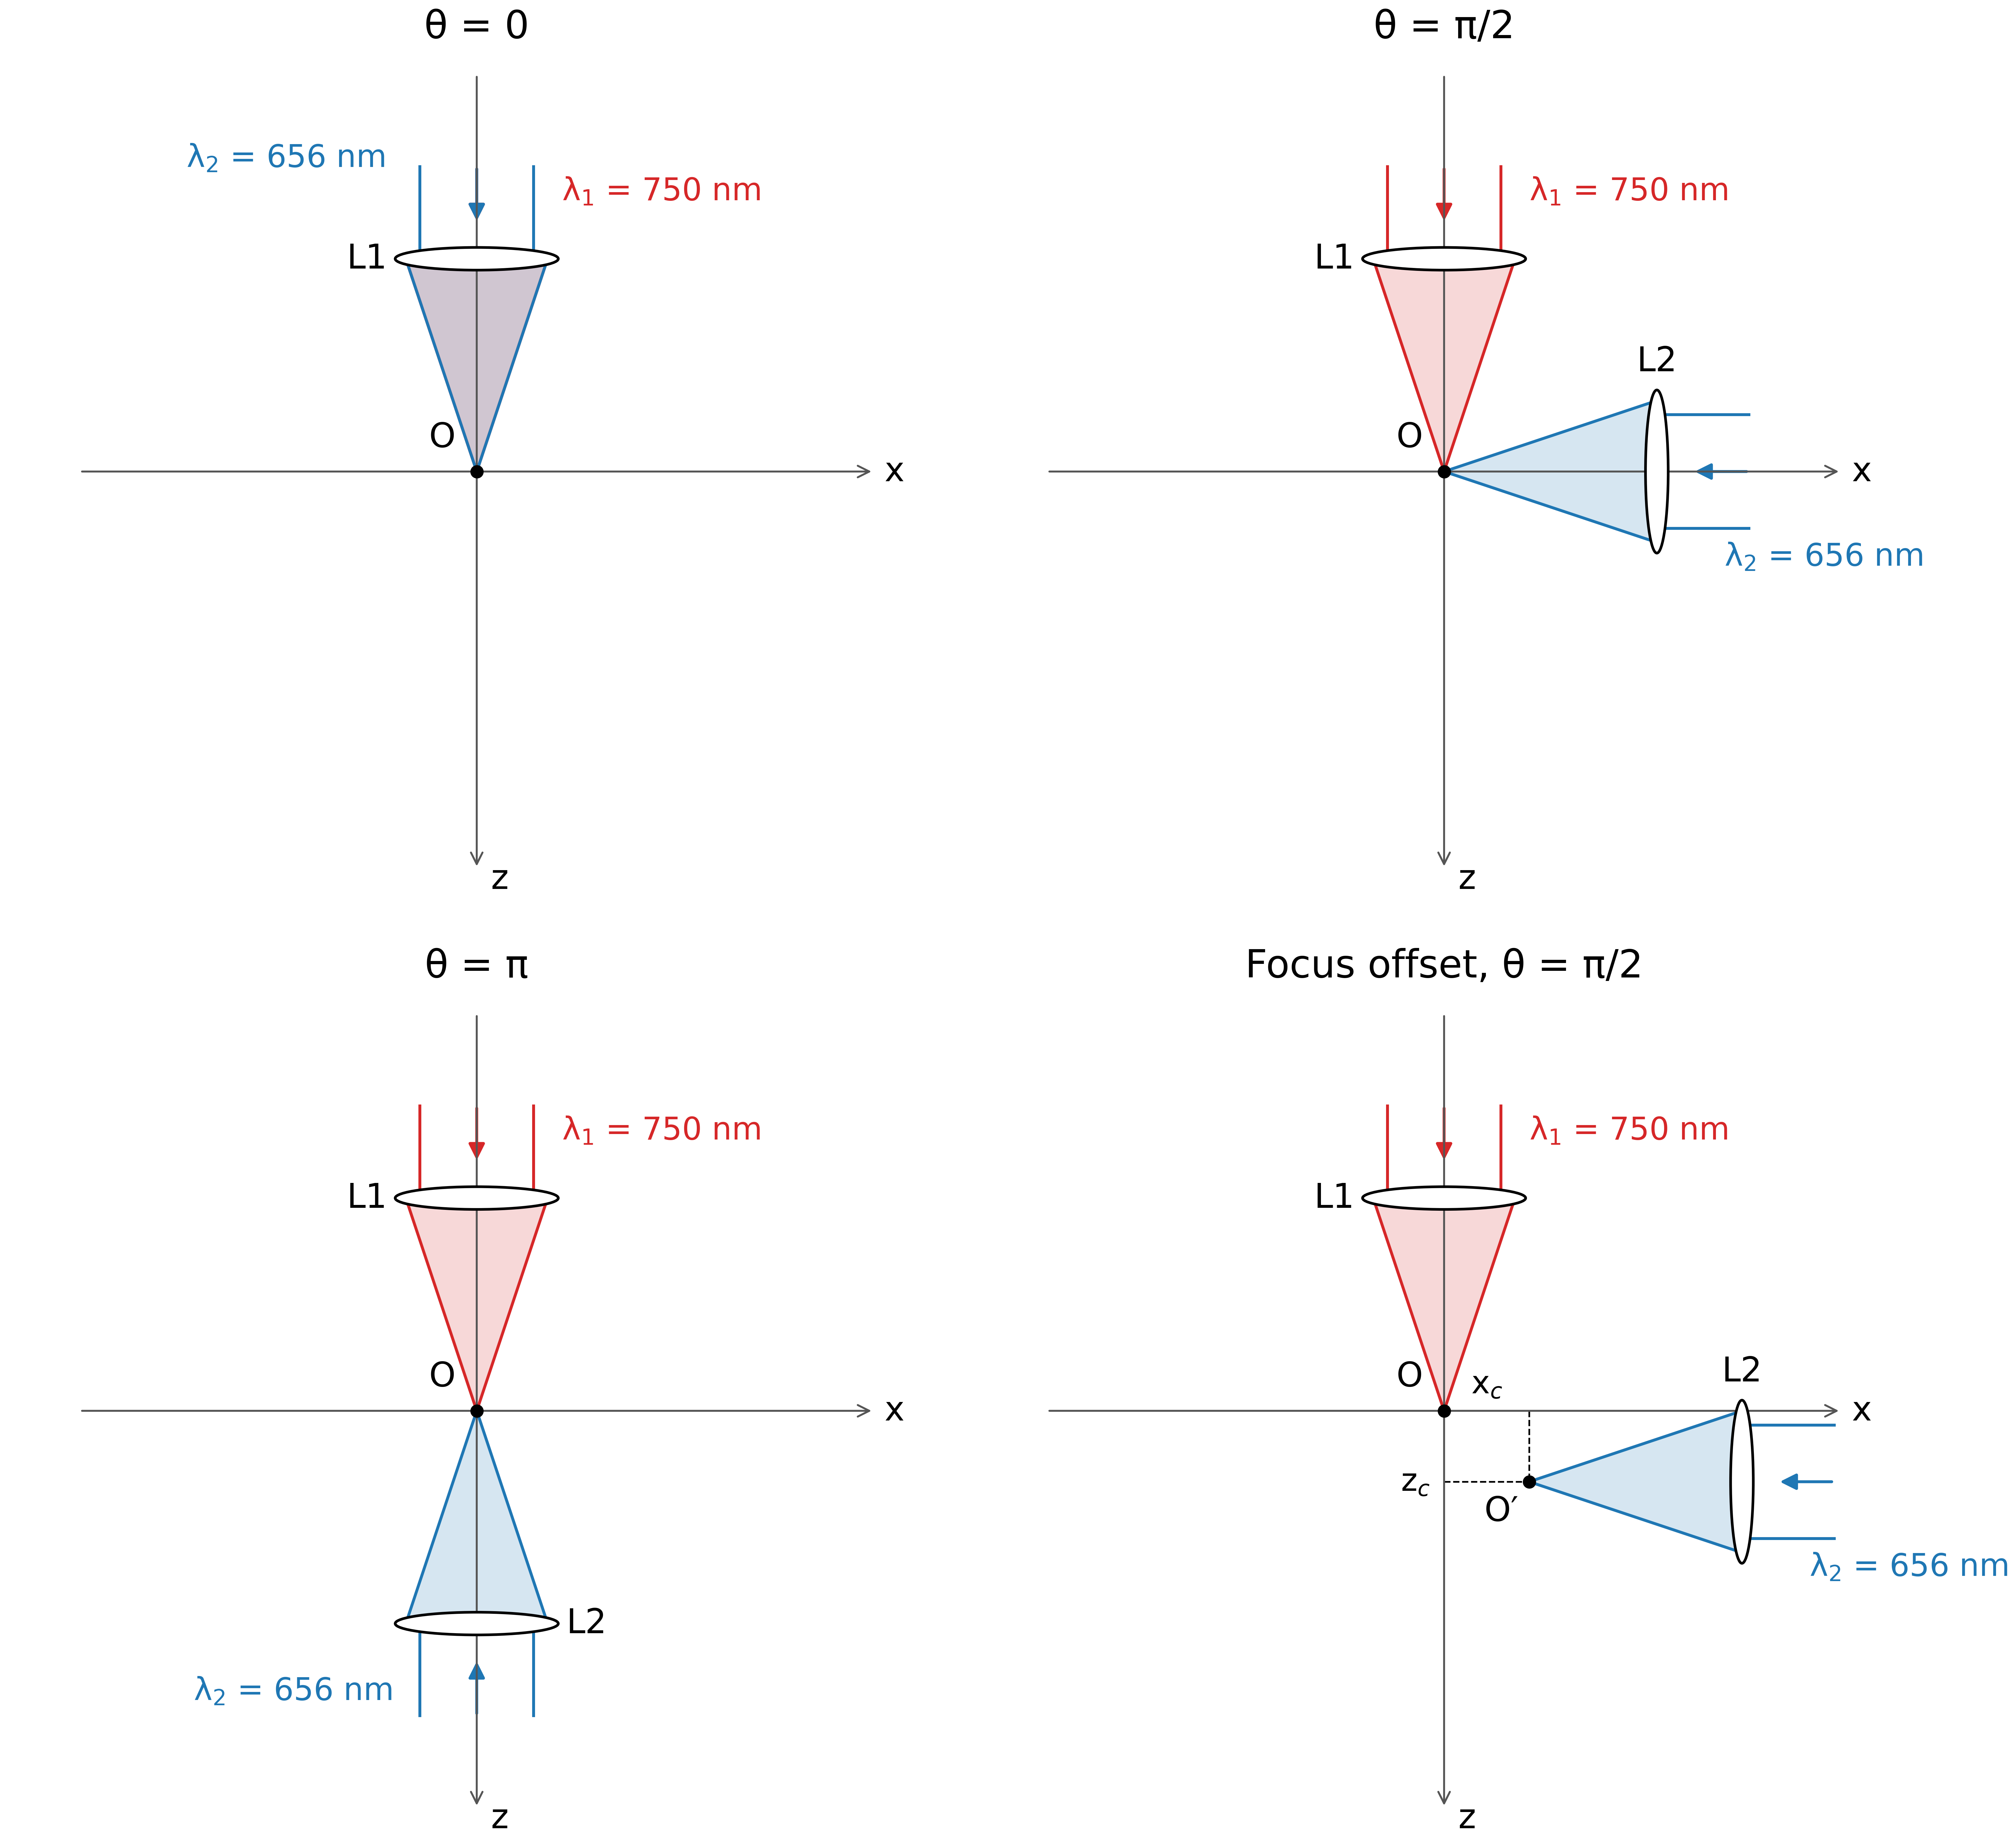
\includegraphics[width=0.58\linewidth]{setup.png}
\caption{Geometry, after \cite{CS00} Fig.~1 and \cite{LS02} Fig.~1: beam 2 rotated by $\theta$, focus moved to
$O'=(x_c,z_c)$.}\label{fig:setup}
\end{figure}

\section{Optical pulses}
A Gaussian pulse of intensity full width $\tau$ has a Gaussian power spectrum of full width
$\Delta\nu=2\ln2/(\pi\tau)\approx0.441/\tau$ \cite{DielsRudolph, Rom03}. Its time-averaged focal intensity is
the spectrum-weighted sum of monochromatic foci, $I(P)=\int S(\omega)\,|\mathbf E(P;\omega)|^2\,d\omega$
\cite{Rom03}, which is what the current pulsed work computes. Two consequences for two-color excitation:
\begin{itemize}
\item At 1\,fs the 750\,nm and 656\,nm spectra share 89\% of their area (Fig.~\ref{fig:pulse}). The cross term
of Section 8 no longer averages away, so few-cycle two-color excitation acquires interference. Lim \& Saloma
report spectral broadening negligible above 10\,fs \cite{LS03}.
\item Two-color excitation needs both pulses at the same place at the same time \cite{LS03}. A 1\,fs pulse is
0.3\,µm long, shorter than the focal region, so a delay between the pulses moves where they meet: time and
position couple.
\end{itemize}

\begin{figure}[H]\centering

\includegraphics[width=\linewidth]{bg_pulse_overlap.png}
\caption{Power spectra of Gaussian pulses centered at 750 and 656\,nm. At 1\,fs they overlap almost
completely; at 20\,fs they are separate.}\label{fig:pulse}
\end{figure}

\part*{II. Replication at low NA}
\noindent\textbf{The three papers.} Cambaliza \& Saloma (2000) \cite{CS00} introduces the comparison: 2CE against
2PE, circular against annular pupils, the wavelength gap $\Delta\lambda$, and a Monte Carlo scattering test, all
with aligned beams. Lim \& Saloma (2002) \cite{LS02} moves beam 2's focus away from beam 1's. Lim \& Saloma (2003)
\cite{LS03} keeps the foci together but gives each beam spherical aberration. Order done here: Lim 2002 first
(it fixed the rotation convention), then Lim 2003 and Cambaliza 2000. All use the paraxial field of Section 6
at NA 0.5, $n=1$, $\lambda_1=750$, $\lambda_2=656$\,nm (2PE at 700\,nm). Code: \texttt{mcdo/twobeam.py}, branch
\texttt{two-color}; the field matches the Airy and $\mathrm{sinc}^2$ profiles to $10^{-10}$.

\begin{center}\small
\begin{tabular}{@{}p{0.29\linewidth}p{0.36\linewidth}p{0.29\linewidth}@{}}
\toprule
Result & Paper & Ours \\ \midrule
\multicolumn{3}{@{}l}{\textbf{Lim \& Saloma 2002} --- focus offset}\\
Peak loss, $\theta=\pi/2$, in plane & $-0.06x_c^2+1$; 11\% at $1.33\lambda_1$ & $-0.063x_c^2+0.999$; 11.1\% \\
Peak loss, $\theta=\pi/2$, axial & $-0.045z_c^2+0.986$; 30\% at $2.7\lambda_1$ & $-0.045z_c^2+0.996$; 31.8\% \\
Peak loss, $\theta=0/\pi$, axial & $-0.027z_c^2+0.996$; 20\% at $2.7\lambda_1$ & $-0.027z_c^2+0.999$; 19.3\% \\
Peak loss, $\theta=0/\pi$, in plane & 20\% at $0.37\lambda_1$ & 17.7\% \\
Linfoot $F$, $\theta=\pi/2$ & stable in plane; $\approx-0.8$ at $z_c=1.33\lambda_1$ & 0.998; $-0.90$ \\
Linfoot $C$, $\theta=\pi/2$ & $\to0$ at $z_c=1.33\lambda_1$ & 1.01 \emph{(not reproduced)} \\
\multicolumn{3}{@{}l}{\textbf{Lim \& Saloma 2003} --- spherical aberration}\\
Peak compensation & along $\phi_1=\phi_2$ ($\theta=0$), $\phi_1=-\phi_2$ ($\pi$) & 0.84 of aligned at $|\phi|=60$ on those lines \\
2CE fidelity, $\theta=\pi/2$ & $F>0.9$ for $|\phi_{1,2}|\le40$ & $F\ge0.928$ \\
Contour maps, Figs.~2--6 & --- & shapes reproduced (Fig.~\ref{fig:rep}) \\
\multicolumn{3}{@{}l}{\textbf{Cambaliza \& Saloma 2000}}\\
FWHM vs $\Delta\lambda$, $\theta=\pi/2$ & data $\approx0.715\to0.757$\,µm & $5.3\times10^{-4}\Delta\lambda+0.713$ \\
DOF vs $\Delta\lambda$, $\theta=\pi/2$ & $-4.81\times10^{-4}\Delta\lambda+0.711$ & $-4.55\times10^{-4}\Delta\lambda+0.713$ \\
Annular 2CE vs circular 2PE, $\theta=0$ & 30\% narrower & 30\% narrower \\
Annular vs circular 2CE, $\theta=\pi/2$ & 32\% narrower & 29\% narrower \\
Spot-size ratios (pp.~28--29) & 0.67, 0.75, 1.58 & 0.49, 0.68, 2.98 \emph{(not reproduced)} \\
Monte Carlo scattering, Fig.~8 & --- & not run (Monte Carlo shelved) \\
\bottomrule
\end{tabular}
\end{center}

\noindent\textbf{Notes.}
(i) Beam 2 must be rotated in real space; the optical-coordinate rotation written in \cite{LS02} (p.~122) gives
$-0.21x_c^2$ instead of $-0.06x_c^2$.
(ii) The caption fit in \cite{CS00} Fig.~5, FWHM $=2.4\times10^{-4}\Delta\lambda+\dots$, disagrees with its own
plotted points ($\approx5\times10^{-4}$); ours follows the points.
(iii) Cambaliza's spot-size ratios fail under FWHM, $1/e^2$ and first-minimum definitions, while its absolute
widths in Fig.~5 match ours; the ratios are treated as unreliable.
(iv) Lim 2002's $C$ map: our $Q$, not $C$, falls to 0.05 at $z_c=1.33\lambda_1$; the labels may be swapped.
(v) With aberration at $\theta=0$ the peak moves to $+z$ under the sign of \cite{LS03} Eq.~1; the paper says
``toward L1''. To check.

\begin{figure}[H]\centering
\includegraphics[width=0.36\linewidth]{psf_aligned_geometric.png}\hfill
\includegraphics[width=0.30\linewidth]{aberration_peak.png}\hfill
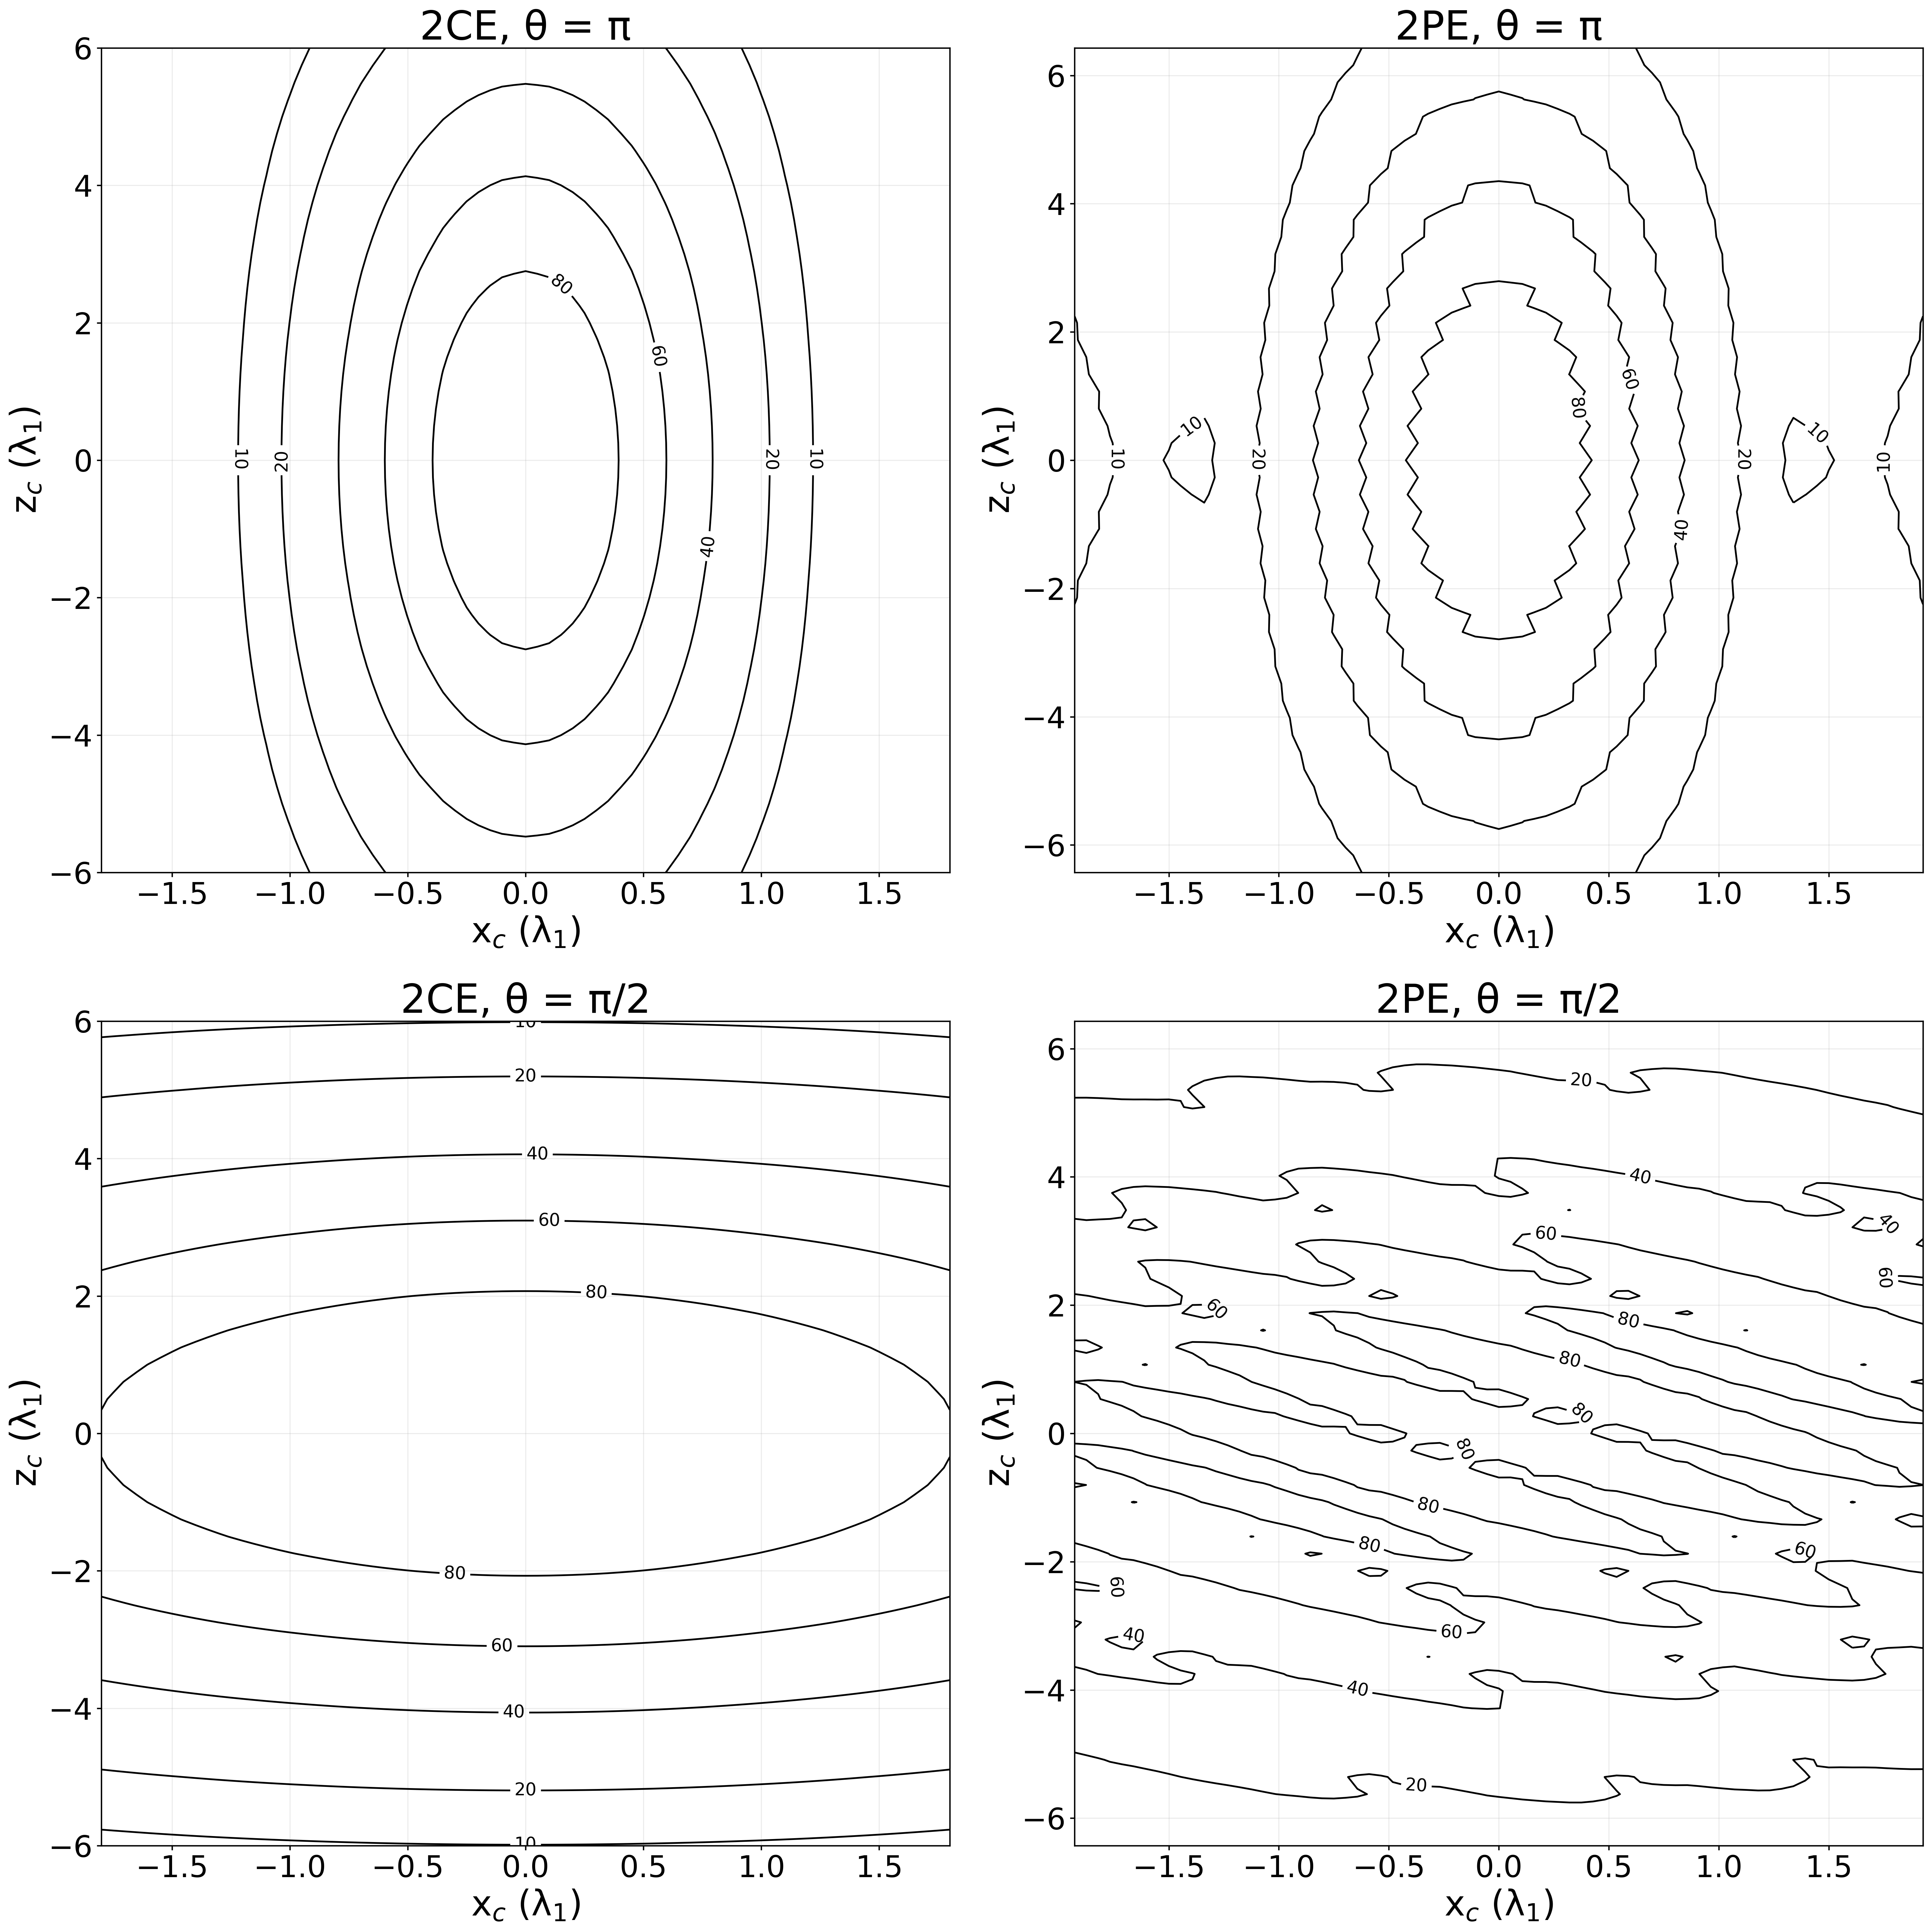
\includegraphics[width=0.30\linewidth]{peak_vs_offset.png}
\caption{Left: aligned 2PE and 2CE point spread functions at $\theta=0,\pi/2,\pi$, after \cite{LS03} Fig.~2.
Center: peak fluorescence (\%) against $\phi_1,\phi_2$, after \cite{LS03} Fig.~4. Right: peak fluorescence
against focus offset, after \cite{LS02} Fig.~4.}\label{fig:rep}
\end{figure}

\part*{III. How it connects to the current work}
\begin{itemize}
\item \textbf{High NA.} The Richards--Wolf engine (Section 5) replaces the paraxial field (Section 6). New
choices appear that the scalar model hides: each beam's polarization, and $E_z$, which rotates with beam 2.
\item \textbf{Geometry.} $\theta=\pi/2$ is limited to NA $\le0.92$ at $n=1.3$; beyond it only $\theta=0,\pi$.
\item \textbf{Annular pupils.} Cambaliza proposes long-DOF annular lenses to keep the foci overlapped
(\cite{CS00} p.~34). The extension law $(1-\cos\alpha)/(\cos\vartheta_{\text{in}}-\cos\alpha)$ and the $\varepsilon$
sweeps quantify that tolerance at high NA.
\item \textbf{Gaussian input.} The truncation parameter $\alpha_t$ enters as each beam's $A(\vartheta)$.
\item \textbf{Pulses.} The spectral integration of Section 10 is already built; at few-cycle durations the
two-color spectra overlap and the no-interference assumption fails.
\item \textbf{Time delay.} Needs the time-resolved field $\mathbf E(P,t)$; the engine currently gives the
time-averaged intensity.
\item \textbf{Metrics.} Linfoot $F$, $C$, $Q$ are already in \texttt{mcdo.linfoot}.
\end{itemize}

\section*{Next steps}
\begin{enumerate}
\item Resolve the open replication items: Lim 2002 $C$ map; aberration sign.
\item The same geometry with the Richards--Wolf field at NA 0.5, choosing polarizations; report the
scalar--vector difference.
\item Raise NA at $\theta=0$ and $\pi$ (and $\pi/2$ up to 0.92); add Gaussian input and annular pupils.
\item Pulsed two-color excitation: spectral overlap and interference at few-cycle durations.
\item Time delay between the pulses: time-resolved fields.
\end{enumerate}

\begin{thebibliography}{99}\small
\bibitem{BornWolf} M. Born and E. Wolf, \emph{Principles of Optics}, 7th (expanded) ed. (Cambridge University
Press, 1999), ISBN 978-0-521-64222-4.
\bibitem{Goodman} J. W. Goodman, \emph{Introduction to Fourier Optics}, 3rd ed. (Roberts \& Company, 2005),
ISBN 978-0-9747077-2-3.
\bibitem{NovotnyHecht} L. Novotny and B. Hecht, \emph{Principles of Nano-Optics} (Cambridge University Press,
2006), ISBN 978-0-521-83224-3.
\bibitem{DielsRudolph} J.-C. Diels and W. Rudolph, \emph{Ultrashort Laser Pulse Phenomena}, 2nd ed.
(Academic Press, 2006), ISBN 978-0-12-215493-5.
\bibitem{Debye} P. Debye, ``Das Verhalten von Lichtwellen in der Nähe eines Brennpunktes oder einer
Brennlinie,'' Ann. Phys. \textbf{335}, 755--776 (1909), doi:10.1002/andp.19093351406.
\bibitem{Wolf59} E. Wolf, ``Electromagnetic diffraction in optical systems I. An integral representation of
the image field,'' Proc. R. Soc. Lond. A \textbf{253}, 349--357 (1959), doi:10.1098/rspa.1959.0199.
\bibitem{RichardsWolf} B. Richards and E. Wolf, ``Electromagnetic diffraction in optical systems II. Structure
of the image field in an aplanatic system,'' Proc. R. Soc. Lond. A \textbf{253}, 358--379 (1959),
doi:10.1098/rspa.1959.0200.
\bibitem{GoeppertMayer} M. Göppert-Mayer, ``Über Elementarakte mit zwei Quantensprüngen,'' Ann. Phys.
\textbf{401}, 273--294 (1931), doi:10.1002/andp.19314010303.
\bibitem{Denk90} W. Denk, J. H. Strickler, and W. W. Webb, ``Two-photon laser scanning fluorescence
microscopy,'' Science \textbf{248}, 73--76 (1990), doi:10.1126/science.2321027.
\bibitem{Lakowicz96} J. R. Lakowicz, I. Gryczynski, H. Malak, and Z. Gryczynski, ``Two-color two-photon
excitation of fluorescence,'' Photochem. Photobiol. \textbf{64}, 632--635 (1996),
doi:10.1111/j.1751-1097.1996.tb03116.x.
\bibitem{Hell92} S. Hell and E. H. K. Stelzer, ``Properties of a 4Pi confocal fluorescence microscope,''
J. Opt. Soc. Am. A \textbf{9}, 2159 (1992), doi:10.1364/JOSAA.9.002159.
\bibitem{Lindek99} S. Lindek and E. H. K. Stelzer, ``Resolution improvement by nonconfocal theta microscopy,''
Opt. Lett. \textbf{24}, 1505--1507 (1999), doi:10.1364/OL.24.001505.
\bibitem{CS00} M. O. Cambaliza and C. Saloma, ``Advantages of two-color excitation fluorescence microscopy with
two confocal excitation beams,'' Opt. Commun. \textbf{184}, 25--35 (2000), doi:10.1016/S0030-4018(00)00929-9.
\bibitem{LS02} M. Lim and C. Saloma, ``Confocality condition in two-color excitation microscopy with two focused
excitation beams,'' Opt. Commun. \textbf{207}, 121--130 (2002), doi:10.1016/S0030-4018(02)01530-4.
\bibitem{LS03} M. Lim and C. Saloma, ``Primary spherical aberration in two-color (two-photon) excitation
fluorescence microscopy with two confocal excitation beams,'' Appl. Opt. \textbf{42}, 3398--3406 (2003),
doi:10.1364/AO.42.003398.
\bibitem{Rom03} K. M. Romallosa, J. Bantang, and C. Saloma, ``Three-dimensional light distribution near the focus
of a tightly focused beam of few-cycle optical pulses,'' Phys. Rev. A \textbf{68}, 033812 (2003),
doi:10.1103/PhysRevA.68.033812.
\end{thebibliography}
\end{document}
